\documentclass[twocolumn, 10pt, a4paper]{article}


%%%%%%%%%%%%%%%%%%%%%%%%%%%%%%%%%
% GETTING STARTED
%%%%%%%%%%%%%%%%%%%%%%%%%%%%%%%%%

% PACKAGES
\usepackage{graphicx}                                                              % figures
\usepackage{natbib}                                                           % bibliography
\usepackage[english]{babel}                         % correct hyphenation (afbreekstreepjes)
\usepackage{url}                                                         % for web addresses

% PAGE MARGINS AND SPACES
\usepackage[top=1.6cm, bottom=2cm, left=1.6cm, right=1.6cm]{geometry}         % page margins
\linespread{1.1}                                                  % more space between lines
\setlength{\parindent}{5mm}                                 % indenting first line paragraph
\setlength{\columnsep}{8mm}                                          % space between columns

% FONT
\usepackage[lf]{berenis}
\renewcommand*\familydefault{\sfdefault} 
\usepackage[T1]{fontenc}


%%%%%%%%%%%%%%%%%%%%%%%%%%%%%%%%%
%%% START
%%%%%%%%%%%%%%%%%%%%%%%%%%%%%%%%%

\begin{document}

% make title
\title{\vspace{-1.4cm} \huge{LaTeX code examples}}
\author{}
\date{}

% print title
\twocolumn[\begin{@twocolumnfalse} \maketitle \end{@twocolumnfalse}]

	
%%%%%%%%%%%%%%%%%%%%%%%%%%%%%%%%%
%%% CONTENTS
%%%%%%%%%%%%%%%%%%%%%%%%%%%%%%%%%


\section{Section header}

\subsection{Subsection header}
\label{sec: header 1}

\subsubsection{Subsubsection header}

\subsubsection*{Subsubsection header without number}

First paragraph 
text text text text text text text text text text text text text text text text 
text text text text text text text text text text text text text text text text
text text text text text text text text text text text text text text text text
text text text text text text text text text text text text text text text text
text text text text text text text text text text text text text text text text

Second paragraph 
text text text text text text text text text text text text text text text text 
text text text text text text text text text text text text text text text text
text text text text text text text text text text text text text text text text
text text text text text text text text text text text text text text text text
text text text text text text text text text text text text text text text text

Third paragraph
text text text text text text text text text text text text text text text text 
text text text text text text text text text text text text text text text text
text text text text text text text text text text text text text text text text
text text text text text text text text text text text text text text text text
text text text text text text text text text text text text text text text text

Fourth paragraph
text text text text text text text text text text text text text text text text 
text text text text text text text text text text text text text text text text
text text text text text text text text text text text text text text text text
text text text text text text text text text text text text text text text text
text text text text text text text text text text text text text text text text


%%%%%%%%%%%%%%%%%%%%%%%%%%%%%%%%%

\section{Figures}

Figures are moved automatically to nice places.

\begin{figure}
	\center
	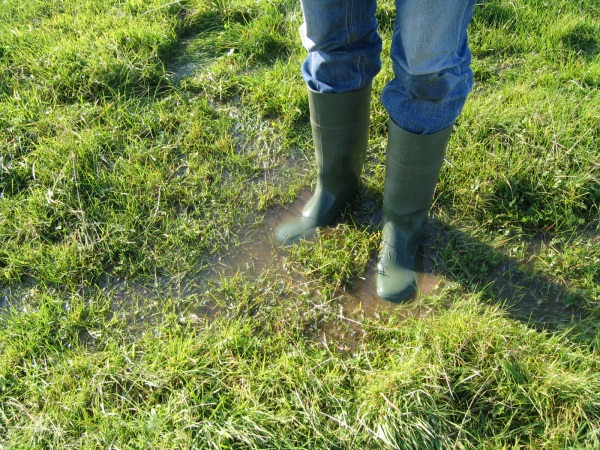
\includegraphics[width=\columnwidth]{figs/ponds.jpg}
	\caption{Single column figure, located in the ``figs'' subdirectory.}
	\label{fig: ponds}
\end{figure}

\begin{figure*}
	\center
	\includegraphics[width=2\columnwidth]{C:/backups/d_schijf/maps/world/GWD/GWD_world_large}
	\caption{Two-column figure located somewhere on my hard drive. This figure will give an error when you compile the tex file yourself, because it will not be able to find it.}
	\label{fig: GWD world}
\end{figure*}


%%%%%%%%%%%%%%%%%%%%%%%%%%%%%%%%%

\section{Tables}

Tables are moved automatically to nice places too. 

If you have many figures and tables compared to text, it sometimes becomes difficult for LaTeX to place them in pretty places. It sometimes helps to move the code for the figure or table in the tex file up or down. Another option is to add \verb|[t]| or \verb|[b]| behind \verb|\begin{figure}| to specify the location (top or bottom of page).


\begin{table}[b]
	\caption{Table with some values. Note the italics for variables and application of subscripts and superscripts.}
	\label{tab: testtable}
	\centering
	\begin{tabular}{lllll}
		\hline
		fit on:&$Q^2$&$Q$&$\sqrt{Q}$&$d_\mathrm{G}$\\
		\hline
		$c_\mathrm{W}$&400&380&379&107\\
		$c_\mathrm{V}$&1.8&0.8&8.2&0.2\\
		$c_\mathrm{G}$&5.3&5.0&5.0&5.0\\
		$c_\mathrm{Q}$&1&4&12&87\\
		\hline
	\end{tabular}
\end{table} 


%%%%%%%%%%%%%%%%%%%%%%%%%%%%%%%%%

\section{Equations}

\begin{equation} 
\label{eq: testequation}
Q = \overline{v} \times A
\end{equation}


%%%%%%%%%%%%%%%%%%%%%%%%%%%%%%%%%

\section{Special characters}

You can use math mode (between dollar signs) for superscripts (x$^\mathsf{2}$) and subscripts (x$_\mathsf{2}$). Italics are default in math mode. If you write in text (so not as an equation), type \verb|\mathsf| to get regular letters.

Variables should always be in italics. Use math mode: $Q$. Units should not be in italics. You can just type them in the text or use \verb|\mathsf| if you have superscripts: $\mathsf{m^{3}\,s^{-1}}$.

Go to \url{detexify.kirelabs.org} to find commands for special characters, such as $\partial$x, $\sqrt{\mathsf{2}}$, etc.


%%%%%%%%%%%%%%%%%%%%%%%%%%%%%%%%%

\section{Lists}

\begin{itemize}
\item first thing
\item second thing
\item third thing
\end{itemize}


%%%%%%%%%%%%%%%%%%%%%%%%%%%%%%%%%

\section{Cross-references} 
\label{sec: header 2}

For cross-references, you have to define a label first (see the \verb|\label| commands above in the tex file). Then you can refer to it using \verb|\ref|:

Refer to Section~\ref{sec: header 2} or Subsection~\ref{sec: header 1}.

Refer to Figure~\ref{fig: GWD world}.

Refer to Table~\ref{tab: testtable}.

Refer to Equation~\ref{eq: testequation}.


%%%%%%%%%%%%%%%%%%%%%%%%%%%%%%%%%

\section{Citation} 
There are several commands to refer to literature, depending on where you want the brackets: 

Floods are important \citep{Brauer2011}.

\cite{Brauer2011} state that floods are important.

Floods are important \citep[according to][]{Brauer2011}.

The bibliography (bib) file should contain entries with the used BiBTeX keys (here \verb!Brauer2011!). The bib file can also contain many more references -- LaTeX will only use the ones to which you refer. 

Adding items to the bibliography file is easy. Option 1: open the .bib file in Notepad, go to Google Scholar, find paper, click "cite", click "import into BiBTeX", copy text into Notepad. Option 2: open the .bib file in JabRef (freely downloadable) and enter more papers. Always check the resulting reference list for errors and missing information. 

Two formatting errors often occur. To keep capitals in the title, put the text between curly brackets. To get long dashes between page numbers (these are often copied wrongly), type \verb|--|. See the example bib file for both. 


%%%%%%%%%%%%%%%%%%%%%%%%%%%%%%%%%
% BIBLIOGRAPHY
%%%%%%%%%%%%%%%%%%%%%%%%%%%%%%%%%

\renewcommand{\bibname}{References} 
\bibliographystyle{elsart-harv}
\bibliography{references_EH}


%%%%%%%%%%%%%%%%%%%%%%%%%%%%%%%%%
% END
%%%%%%%%%%%%%%%%%%%%%%%%%%%%%%%%%

\end{document}
